% =============================================================================
% Capítulo 5 — Resultados
% =============================================================================
% Este capítulo apresenta os resultados dos experimentos de classificação
% binária para detecção de ocultações estelares em curvas de luz, em conformidade
% com a metodologia descrita no Capítulo 4.

\section{Visão geral dos experimentos}
\label{sec:visao_geral_resultados}

Este capítulo apresenta os resultados obtidos com a \textit{pipeline} de detecção automatizada de ocultações estelares em curvas de luz, descrita no Capítulo~4. O problema é formulado como \textbf{classificação binária}: cada curva é rotulada como \textbf{positiva} (evento de ocultação presente) ou \textbf{negativa} (ausência de evento). Foram treinados e avaliados quatro classificadores --- Regressão Logística, Random Forest, XGBoost e CatBoost --- cujo desempenho foi medido exclusivamente no \textbf{conjunto de teste}, isto é, em dados que não participaram do treinamento.

As métricas adotadas são: \textbf{acurácia} (fração de acertos no total), \textbf{precisão} (entre as curvas classificadas como positivas, quantas eram realmente positivas), \textbf{sensibilidade} ou \textit{recall} (entre todas as curvas realmente positivas, quantas foram detectadas), \textbf{F1-score} (média harmônica entre precisão e sensibilidade) e \textbf{área sob a curva ROC} (AUC-ROC), que resume a capacidade do modelo de separar as duas classes para diversos limiares de decisão. As \textbf{matrizes de confusão} mostram quantos verdadeiros positivos (TP), verdadeiros negativos (TN), falsos positivos (FP) e falsos negativos (FN) cada modelo produziu.

A montagem de um conjunto de dados equilibrado foi a primeira grande dificuldade do projeto: nos catálogos disponíveis (VizieR, Grupo do Rio), o número de curvas negativas é muito inferior ao de positivas --- o banco dispunha de 802 curvas positivas e apenas 3 negativas. Para contornar esse desbalanceamento, adotaram-se duas estratégias complementares, descritas no Capítulo~4: recorte de segmentos sem ocultação a partir das curvas positivas (com revisão manual), gerando 186 negativos artificiais, e incorporação de 702 curvas sintéticas negativas geradas pelo simulador físico de Gomes-Ferrante \& Braga-Ribas~\citep{Simulator}. O \textit{dataset} final reúne \textbf{1693 amostras} (802 positivas e 891 negativas), com divisão treino/teste estratificada por curva (80\%/20\%).

Ao todo, foram realizados \textbf{seis experimentos}, que variam o conjunto de \textit{features} (de 28 a 11 variáveis) e a composição do conjunto de teste (misto ou exclusivamente real). Como o desempenho se mostrou notavelmente estável entre eles, este capítulo apresenta \textbf{em detalhe os três experimentos mais informativos}, que sintetizam a progressão lógica do trabalho:

\begin{itemize}
	\item \textbf{Experimento 1:} conjunto completo de 28 \textit{features}, divisão 80\%/20\%. É a \textbf{linha de base} de desempenho, com todas as variáveis disponíveis.
	\item \textbf{Experimento 2:} 11 \textit{features} (sem \texttt{Feature\_Savgol\_Min} e sem \texttt{kmeans\_centroid\_dist}), divisão 80\%/20\%. É a \textbf{configuração enxuta} adotada como referência operacional --- a mais simples sem perda de desempenho, e a usada no estudo de caso de Quaoar.
	\item \textbf{Experimento 3:} 11 \textit{features}, porém com \textbf{teste somente em curvas reais} (excluindo as sintéticas). É o teste de \textbf{generalização} mais próximo do uso real.
\end{itemize}

Os demais três experimentos --- a redução intermediária de \textit{features} para 14 (Experimento 4) e 13 variáveis (Experimento 5) e a ablação isolada da \textit{feature} \texttt{kmeans\_centroid\_dist} (Experimento 6) --- conduzem às mesmas conclusões e estão documentados em detalhe no Apêndice~\ref{ap:experimentos}. Suas métricas são consolidadas, ao lado das dos três experimentos-destaque, na Tabela~\ref{tab:comparacao_f1} (Seção~\ref{sec:comparacao}).

Em todos os experimentos, o mesmo protocolo foi aplicado: divisão treino/teste estratificada, preenchimento de valores faltantes pela mediana calculada no treino, e padronização das características (média zero, desvio unitário) apenas para a Regressão Logística, conforme detalhado no Capítulo~4.

Além dos experimentos de classificação, este capítulo apresenta uma análise de \textbf{ajuste do limiar de decisão} (Seção~\ref{sec:threshold_tuning}), que investiga como reduzir o limiar de classificação para minimizar falsos negativos --- uma demanda natural em cenários de triagem científica, onde perder uma ocultação real é mais custoso do que revisar um falso alarme. Por fim, um \textbf{estudo de caso} (Seção~\ref{sec:estudo_caso_quaoar}) aplica a \textit{pipeline} a curvas reais de uma ocultação estelar pelo objeto transnetuniano (50000) Quaoar~\citep{Quaoar2023} --- dados externos ao banco de treino e morfologicamente complexos (corpo principal e estruturas de anel) --- como teste de generalização operacional e como demonstração da capacidade de revisitar curvas em busca de eventos sutis.

% -----------------------------------------------------------------------------
\section{Descrição das \textit{features} e análise de redundância}
\label{sec:features_redundancia}

\subsection{Conjunto completo de \textit{features}}

A \textit{pipeline} de extração de características produz 28 variáveis numéricas a partir de cada curva de luz normalizada. Essas variáveis podem ser agrupadas em cinco famílias, descritas na Tabela~\ref{tab:features_completo}.

\begin{table}[htbp]
\centering
\caption{Conjunto completo de 28 \textit{features} extraídas pela \textit{pipeline}. A coluna ``Família'' indica o grupo funcional; a coluna ``Definição'' resume o cálculo.}
\label{tab:features_completo}
\footnotesize
\begin{tabular}{llp{7.5cm}}
\hline
\textbf{Família} & \textbf{Feature} & \textbf{Definição} \\
\hline
\multirow{3}{*}{Fluxo bruto}
& \texttt{Feature\_Amp} & $\max(f) - \min(f)$ (amplitude total do fluxo) \\
& \texttt{Feature\_Flux\_std} & $\sigma(f)$ (desvio padrão do fluxo) \\
& \texttt{Max\_Drawdown} & $\min(f_i - \max_{j \le i} f_j)$ (maior queda acumulada) \\
\hline
\multirow{3}{*}{Savitzky-Golay}
& \texttt{Feature\_Savgol\_Max} & $\max(\tilde{f})$ (máximo do fluxo suavizado) \\
& \texttt{Feature\_Savgol\_Min} & $\min(\tilde{f})$ (mínimo do fluxo suavizado) \\
& \texttt{Feature\_Savgol\_std} & $\sigma(\tilde{f})$ (desvio padrão do fluxo suavizado) \\
\hline
K-Means & \texttt{kmeans\_centroid\_dist} & Distância entre os 2 centróides do K-Means aplicado a $\tilde{f}$ \\
\hline
\multirow{2}{*}{Testes de quartis}
& \texttt{MinLogP\_Ttest} & $-\log_{10}(\min p_{\text{t-test}})$ entre pares de quartis \\
& \texttt{MinLogP\_KS} & $-\log_{10}(\min p_{\text{KS}})$ entre pares de quartis \\
\hline
\multirow{9}{*}{Derivadas}
& \texttt{Deriv\_Min} & $\min(f')$ \\
& \texttt{Deriv\_Max} & $\max(f')$ \\
& \texttt{Deriv\_Mean} & $\bar{f'}$ \\
& \texttt{Deriv\_Std} & $\sigma(f')$ \\
& \texttt{Deriv\_Skew} & Assimetria de $f'$ \\
& \texttt{Deriv\_Kurtosis} & Curtose de $f'$ \\
& \texttt{SecondDeriv\_Min} & $\min(f'')$ \\
& \texttt{SecondDeriv\_Max} & $\max(f'')$ \\
& \texttt{SecondDeriv\_Std} & $\sigma(f'')$ \\
\hline
\multirow{10}{*}{Observacionais}
& \texttt{Occ\_depth} & $\text{baseline} - \min(f)$ (profundidade do dip) \\
& \texttt{Occ\_SNR\_dip} & $\text{depth}/\sigma_{\text{baseline}}$ (razão sinal-ruído do dip) \\
& \texttt{Occ\_duration\_s} & Duração do maior bloco abaixo do baseline (em segundos) \\
& \texttt{Occ\_n\_frames\_below\_baseline} & Maior nº de frames consecutivos abaixo do baseline \\
& \texttt{Occ\_baseline\_std} & $\sigma(f \mid f \ge \text{baseline})$ (ruído fora do dip) \\
& \texttt{Occ\_flux\_min} & $\min(f)$ \\
& \texttt{Occ\_flux\_min\_over\_baseline} & $\min(f)/\text{baseline}$ \\
& \texttt{Occ\_chi2\_constant} & $\chi^2$ do modelo constante (sem evento) \\
& \texttt{Occ\_chi2\_square\_well} & $\chi^2$ do modelo de poço retangular \\
& \texttt{Occ\_chi2\_ratio} & $\chi^2_{\text{const}}/\chi^2_{\text{sw}}$ (razão de ajuste) \\
\hline
\end{tabular}
\end{table}

Nas definições acima, $f$ denota o vetor de fluxo normalizado, $\tilde{f}$ o fluxo suavizado por filtro Savitzky-Golay (polinômio de grau 2, janela adaptativa), $f'$ e $f''$ a primeira e segunda derivadas numéricas de $\tilde{f}$, e \emph{baseline} a mediana de $f$.

\subsection{Análise de redundância}

A presença de variáveis redundantes --- altamente correlacionadas ou conceitualmente equivalentes --- pode inflar a dimensionalidade sem acrescentar informação discriminativa, aumentar o risco de \textit{overfitting} e dificultar a interpretação da importância das \textit{features}. Para identificar pares redundantes, foram analisadas tanto as definições matemáticas quanto as correlações empíricas entre as 28 variáveis. Os pares identificados são apresentados a seguir.

\begin{enumerate}
	\item \textbf{\texttt{Feature\_Amp} vs.\ \texttt{Occ\_depth}.}
	A amplitude é definida como $\max(f) - \min(f)$, enquanto a profundidade observacional é $\text{baseline} - \min(f)$, com $\text{baseline} = \text{mediana}(f)$. Para curvas de fluxo normalizado próximo de 1, o máximo tende a coincidir com a mediana, tornando as duas métricas praticamente idênticas. \textbf{Removida:} \texttt{Feature\_Amp}. \textbf{Mantida:} \texttt{Occ\_depth}, por possuir motivação física direta na caracterização de ocultações.

	\item \textbf{\texttt{Feature\_Flux\_std} vs.\ \texttt{Occ\_baseline\_std}.}
	O desvio padrão do fluxo total ($\sigma(f)$) inclui os pontos dentro do dip, inflando a medida de ruído quando há ocultação. O desvio padrão do \textit{baseline} ($\sigma(f \mid f \ge \text{mediana})$) estima o ruído fotométrico fora do evento, sendo mais adequado fisicamente. \textbf{Removida:} \texttt{Feature\_Flux\_std}. \textbf{Mantida:} \texttt{Occ\_baseline\_std}.

	\item \textbf{\texttt{Occ\_flux\_min} vs.\ \texttt{Feature\_Savgol\_Min}.}
	O mínimo do fluxo bruto e o mínimo do fluxo suavizado por Savitzky-Golay são altamente correlacionados, pois o filtro preserva a posição dos mínimos. A versão suavizada é mais robusta a ruído pontual. \textbf{Removida:} \texttt{Occ\_flux\_min}. \textbf{Mantida:} \texttt{Feature\_Savgol\_Min}.

	\item \textbf{\texttt{Occ\_flux\_min\_over\_baseline}.}
	Esta razão ($\min(f)/\text{baseline}$) é algebricamente derivável de \texttt{Occ\_depth} e do valor do \textit{baseline}, não acrescentando informação independente. \textbf{Removida.}

	\item \textbf{\texttt{Occ\_n\_frames\_below\_baseline} vs.\ \texttt{Occ\_duration\_s}.}
	Para observações com cadência uniforme, a duração em segundos é proporcional ao número de frames ($\Delta t_{\text{dur}} \approx n_{\text{frames}} \times \delta t$). A duração em unidade física (segundos) é mais interpretável e invariante a mudanças de cadência. \textbf{Removido:} \texttt{Occ\_n\_frames\_below\_baseline}. \textbf{Mantida:} \texttt{Occ\_duration\_s}.

	\item \textbf{\texttt{Feature\_Savgol\_Max}.}
	Para fluxo normalizado, o máximo do sinal suavizado é próximo de 1,0 em quase todas as curvas, resultando em variância muito baixa e poder discriminativo desprezível. \textbf{Removida.}

	\item \textbf{Nove \textit{features} de derivadas (\texttt{Deriv\_*} e \texttt{SecondDeriv\_*}).}
	No Experimento 4, a remoção das nove \textit{features} de derivadas não causou perda de desempenho (F1 mantido em 0,99). Além disso, as métricas observacionais de profundidade, duração e razão $\chi^2$ já capturam as variações abruptas do fluxo que as derivadas buscam codificar, caracterizando redundância conceitual. \textbf{Removidas} todas as nove variáveis de derivadas.
\end{enumerate}

Após a remoção, o conjunto final utilizado no treinamento contém \textbf{13 \textit{features}}, listadas na Tabela~\ref{tab:features_final}.

\begin{table}[htbp]
\centering
\caption{Conjunto final de 13 \textit{features} após remoção de redundâncias.}
\label{tab:features_final}
\begin{tabular}{ll}
\hline
\textbf{Família} & \textbf{Feature} \\
\hline
Savitzky-Golay & \texttt{Feature\_Savgol\_Min}, \texttt{Feature\_Savgol\_std} \\
Fluxo bruto & \texttt{Max\_Drawdown} \\
K-Means & \texttt{kmeans\_centroid\_dist} \\
Testes de quartis & \texttt{MinLogP\_Ttest}, \texttt{MinLogP\_KS} \\
\multirow{2}{*}{Observacionais} & \texttt{Occ\_depth}, \texttt{Occ\_SNR\_dip}, \texttt{Occ\_duration\_s} \\
& \texttt{Occ\_baseline\_std}, \texttt{Occ\_chi2\_constant}, \texttt{Occ\_chi2\_square\_well}, \texttt{Occ\_chi2\_ratio} \\
\hline
\end{tabular}
\end{table}

É importante ressaltar que as 15 variáveis removidas \textbf{continuam sendo calculadas e armazenadas} no arquivo CSV do \textit{dataset}. A exclusão ocorre apenas no momento do treinamento, por meio de uma lista configurável no código (\texttt{EXCLUDED\_FEATURES}). Essa decisão de projeto permite re-incluir qualquer variável em estudos futuros de ablação sem necessidade de reprocessar as curvas de luz.

% -----------------------------------------------------------------------------
\section{Importância das \textit{features}: metodologia}
\label{sec:feature_importance_metodologia}

Uma das vantagens de modelos baseados em árvores e de modelos lineares é a possibilidade de quantificar a contribuição individual de cada variável para a decisão do classificador. Entretanto, cada família de modelos emprega uma definição distinta de ``importância'', e valores obtidos por métodos diferentes \textbf{não devem ser comparados diretamente em escala absoluta}. Esta seção descreve o cálculo adotado internamente por cada um dos quatro classificadores utilizados neste trabalho.

\subsection{Random Forest --- \textit{Mean Decrease in Impurity} (MDI)}

O Random Forest é um \textit{ensemble} de árvores de decisão. Cada nó de cada árvore realiza uma divisão (\textit{split}) em uma variável, e essa divisão reduz a impureza (medida pelo índice de Gini) dos subconjuntos resultantes. Para uma \textit{feature} $x_j$, a importância MDI é definida como a \textbf{média}, sobre todas as árvores e todos os nós, da redução de impureza atribuída a $x_j$:
%
\[
\text{MDI}(x_j) \;=\; \frac{1}{T}\sum_{t=1}^{T}\sum_{n \in \mathcal{N}_t(x_j)} \Delta I(n),
\]
%
onde $T$ é o número de árvores, $\mathcal{N}_t(x_j)$ é o conjunto de nós da árvore $t$ que utilizam $x_j$ para o \textit{split}, e $\Delta I(n)$ é a redução ponderada de impureza no nó $n$.

Na implementação do \texttt{scikit-learn}, os valores de MDI são \textbf{normalizados para que a soma seja igual a~1}. Consequentemente, com 13 \textit{features}, nenhuma variável individual ultrapassa tipicamente valores de importância em torno de 0,20--0,30, e o eixo horizontal dos gráficos de importância varia de~0 a~$\approx$0,25.

Uma limitação conhecida do MDI é o viés em favor de variáveis contínuas de alta cardinalidade, que oferecem mais candidatos para \textit{split}.

\subsection{XGBoost --- \textit{Weight} (contagem de \textit{splits})}

O XGBoost constrói árvores de forma sequencial por \textit{gradient boosting}. Na interface do \texttt{scikit-learn} (\texttt{XGBClassifier}), o atributo \texttt{feature\_importances\_} retorna, por padrão, a métrica \textbf{\textit{weight}}: para cada \textit{feature} $x_j$, conta-se o número total de vezes em que $x_j$ foi selecionada como variável de \textit{split} em todas as árvores do \textit{ensemble}. Os valores são então normalizados para somar~1.

A métrica \textit{weight} mede a \textbf{frequência de uso} da variável, não a magnitude da melhoria que cada \textit{split} proporciona. Alternativas disponíveis no XGBoost incluem \textit{gain} (melhoria média de perda) e \textit{cover} (número médio de amostras afetadas). Neste trabalho, utilizou-se o \textit{weight} padrão.

\subsection{CatBoost --- \textit{PredictionValuesChange}}

O CatBoost, assim como o XGBoost, é um algoritmo de \textit{gradient boosting}. Porém, a métrica de importância padrão retornada por \texttt{feature\_importances\_} é o \textbf{\textit{PredictionValuesChange}}: para cada \textit{feature} $x_j$, calcula-se a mudança média no valor de predição do modelo quando os valores de $x_j$ são permutados aleatoriamente. Essa abordagem é conceitualmente próxima da \textbf{importância por permutação}, sendo mais fidedigna à contribuição preditiva real da variável do que métricas baseadas em contagem de \textit{splits}.

Os valores de \textit{PredictionValuesChange} são normalizados para somar~100 na implementação do CatBoost, de modo que a escala dos gráficos difere da adotada pelo Random Forest e XGBoost.

\subsection{Regressão Logística --- valor absoluto dos coeficientes}

Na Regressão Logística, cada \textit{feature} $x_j$ possui um coeficiente $\beta_j$ no modelo log-linear:
%
\[
\log\frac{P(y=1)}{P(y=0)} = \beta_0 + \sum_{j=1}^{p} \beta_j\,x_j.
\]
%
Como as \textit{features} são previamente padronizadas (média zero, desvio unitário) pelo \texttt{StandardScaler}, os coeficientes estão em escalas comparáveis. A importância de $x_j$ é então estimada como $|\beta_j|$: quanto maior o módulo do coeficiente, maior a influência da variável na probabilidade de ocultação.

Ao contrário dos modelos baseados em árvores, esses valores \textbf{não são normalizados para somar 1 ou 100}, e por isso a escala do gráfico pode variar de 0 a valores como 3 ou 4, dependendo do problema.

\subsection{Comparação entre os métodos}

A Tabela~\ref{tab:metodos_importancia} sintetiza as diferenças entre os quatro métodos.

\begin{table}[htbp]
\centering
\caption{Comparação dos métodos de cálculo de importância de \textit{features} utilizados por cada modelo.}
\label{tab:metodos_importancia}
\footnotesize
\begin{tabular}{llcc}
\hline
\textbf{Modelo} & \textbf{Métrica} & \textbf{Normalização} & \textbf{Escala típica} \\
\hline
Random Forest & MDI (Gini) & $\sum = 1$ & 0 a $\approx$0,25 \\
XGBoost & \textit{Weight} (contagem de \textit{splits}) & $\sum = 1$ & 0 a $\approx$0,15 \\
CatBoost & \textit{PredictionValuesChange} & $\sum = 100$ & 0 a $\approx$30 \\
Regressão Logística & $|\beta_j|$ (coeficientes) & Sem normalização & 0 a $\approx$4 \\
\hline
\end{tabular}
\end{table}

É fundamental notar que \textbf{a mesma \textit{feature} pode ter importância relativa diferente entre modelos}, sem que isso represente contradição: cada algoritmo captura padrões distintos nos dados, e a métrica de importância reflete a forma como cada modelo utiliza internamente a variável. A análise de importância, portanto, deve ser interpretada dentro de cada modelo, e não como um \textit{ranking} absoluto.

% -----------------------------------------------------------------------------
\section{Configuração experimental}
\label{sec:config_experimental}

Para os experimentos foram processadas \textbf{802 curvas positivas} do banco de dados (VizieR e Grupo do Rio); a partir delas, foram obtidos \textbf{186 negativos artificiais} por recorte manual de segmentos sem ocultação. Além disso, foram utilizadas \textbf{3 curvas negativas} do próprio banco e \textbf{702 curvas sintéticas negativas} geradas pelo simulador de Gomes-Ferrante \& Braga-Ribas~\citep{Simulator}. A Tabela~\ref{tab:dataset_fonte} resume a composição do \textit{dataset}.

\begin{table}[htbp]
\centering
\caption{Distribuição das amostras por fonte no \textit{dataset} utilizado nos experimentos.}
\label{tab:dataset_fonte}
\begin{tabular}{lc}
\hline
\textbf{Fonte} & \textbf{Quantidade} \\
\hline
Curvas positivas do banco (db\_positive)   & 802 \\
Curvas sintéticas negativas (synthetic)    & 702 \\
Negativos artificiais (recorte manual)    & 186 \\
Curvas negativas do banco (db\_negative)  & 3 \\
\hline
\textbf{Total} & 1693 \\
\hline
\end{tabular}
\end{table}

A divisão entre treino e teste foi feita de forma \textbf{estratificada por curva} (80\% treino, 20\% teste): cada curva aparece integralmente em treino ou em teste, nunca nos dois, evitando vazamento de informação. O conjunto de teste contém 339 curvas (aproximadamente 178--179 negativas e 160--161 positivas).

Os hiperparâmetros (número de árvores, profundidade máxima, regularização, etc.) foram fixados conforme o Apêndice~\ref{ap:hiperparametros}. Utilizou-se ponderação das classes nos quatro algoritmos para lidar com o desbalanceamento residual. A semente aleatória foi fixada em 42 para reprodutibilidade. Todas as métricas referem-se exclusivamente ao \textbf{conjunto de teste}.

% -----------------------------------------------------------------------------
\section{Resultados do Experimento 1 (linha de base, 28 \textit{features})}
\label{sec:resultados_exp1}

No Experimento 1 foram utilizadas as 28 \textit{features} descritas na Tabela~\ref{tab:features_completo} (conjunto completo). A Tabela~\ref{tab:metricas_1} resume as métricas de desempenho no conjunto de teste.

\begin{table}[htbp]
\centering
\caption{Métricas de desempenho no conjunto de teste --- Experimento 1. Conjunto completo de 28 \textit{features}, divisão 80\%/20\%.}
\label{tab:metricas_1}
\begin{tabular}{lccccc}
\hline
\textbf{Modelo} & \textbf{Acurácia} & \textbf{Precisão} & \textbf{Sensibilidade} & \textbf{F1-score} & \textbf{AUC-ROC} \\
\hline
Random Forest   & \textbf{0,9941} & 1,0000 & 0,9875 & \textbf{0,9937} & 0,9997 \\
CatBoost        & 0,9912 & 0,9937 & 0,9875 & 0,9906 & 0,9998 \\
Regressão Log.  & 0,9882 & 1,0000 & 0,9750 & 0,9873 & 1,0000 \\
XGBoost         & 0,9853 & 0,9814 & 0,9875 & 0,9844 & 0,9997 \\
\hline
\end{tabular}
\end{table}

O melhor desempenho em F1-score e acurácia foi obtido pelo \textbf{Random Forest} (F1 = 0,9937; acurácia = 0,9941). A sensibilidade de 98,75\% indica que a grande maioria das curvas com ocultação foi corretamente identificada; a precisão de 100\% indica ausência de falsos positivos nesse modelo. A Regressão Logística também alcança precisão de 100\%. A AUC-ROC muito alta ($\geq 0{,}9997$) confirma excelente capacidade de separação das classes.

A Figura~\ref{fig:confusao_1} apresenta as matrizes de confusão dos quatro modelos no Experimento 1.

\begin{figure}[htbp]
\begin{center}
	
\includegraphics[width=0.85\textwidth]{Tese/pngs/exp1/confusion_matrices.png}
\caption{Matrizes de confusão dos quatro modelos no Experimento 1 (28 \textit{features}). Eixos: real (vertical) e predito (horizontal). Classes: Negativa~(0) e Positiva~(1).}
\label{fig:confusao_1}
\end{center}
\end{figure}

% -----------------------------------------------------------------------------
\section{Redução do conjunto de \textit{features}: da linha de base à configuração enxuta}
\label{sec:ablation_kmeans}

Partindo das 28 \textit{features} do Experimento~1, o conjunto de variáveis foi progressivamente reduzido, removendo aquelas identificadas como redundantes ou pouco discriminativas (Seção~\ref{sec:features_redundancia}). O Experimento~4 (14 \textit{features}) elimina amplitude, desvio padrão do fluxo bruto, máximo do Savitzky-Golay e as derivadas; o Experimento~5 (13 \textit{features}) remove adicionalmente \texttt{Feature\_Savgol\_Min}; e o Experimento~6 (12 \textit{features}) ablaciona a \texttt{kmeans\_centroid\_dist}. Em todos eles, o melhor F1-score permanece em torno de 0,99 --- ou seja, \textbf{a remoção dessas variáveis não degrada o desempenho}. Os resultados completos desses três experimentos (tabelas e matrizes de confusão) estão no Apêndice~\ref{ap:experimentos}; a Tabela~\ref{tab:comparacao_f1} (Seção~\ref{sec:comparacao}) consolida os valores.

Um achado merece destaque por ser, à primeira vista, contraintuitivo. A \texttt{kmeans\_centroid\_dist} --- distância entre os dois centróides obtidos pela aplicação de K-Means ($K=2$) ao fluxo suavizado --- figura consistentemente entre as variáveis \emph{mais importantes} nos modelos de árvore, chegando a concentrar boa parte da importância no XGBoost. Ainda assim, removê-la (Experimento~6) \textbf{não piora o desempenho}: a capacidade preditiva é simplesmente redistribuída para variáveis colineares, sobretudo \texttt{Feature\_Savgol\_std} --- que captura o mesmo fenômeno físico, a dispersão do fluxo causada pelos dois patamares dentro e fora do \textit{dip}. A lição é importante: \textbf{a importância atribuída por um algoritmo de árvore não é sinônimo de insubstituibilidade}; uma variável pode concentrar importância apenas por oferecer um ponto de corte conveniente, enquanto outras compensam sua ausência. Na prática, isso permite simplificar a \textit{pipeline} eliminando o passo de K-Means sem custo de desempenho.

\subsection{Configuração enxuta: Experimento 2 (11 \textit{features})}
\label{sec:resultados_exp5}

O Experimento~2 leva essa simplificação ao limite, removendo \emph{simultaneamente} \texttt{Feature\_Savgol\_Min} e \texttt{kmeans\_centroid\_dist} e restando \textbf{11 \textit{features}}, com divisão 80\%/20\%. É esta a \textbf{configuração enxuta} adotada como referência operacional do trabalho --- a mais simples que preserva o desempenho da linha de base --- e a empregada no estudo de caso de Quaoar (Seção~\ref{sec:estudo_caso_quaoar}). A Tabela~\ref{tab:metricas_5} apresenta as métricas.

\begin{table}[htbp]
\centering
\caption{Métricas de desempenho no conjunto de teste --- Experimento 2. 11 \textit{features} (sem \texttt{Feature\_Savgol\_Min} e sem \texttt{kmeans\_centroid\_dist}), divisão 80\%/20\%.}
\label{tab:metricas_5}
\begin{tabular}{lccccc}
\hline
\textbf{Modelo} & \textbf{Acurácia} & \textbf{Precisão} & \textbf{Sensibilidade} & \textbf{F1-score} & \textbf{AUC-ROC} \\
\hline
XGBoost         & \textbf{0,9912} & 0,9937 & 0,9875 & \textbf{0,9906} & 0,9995 \\
CatBoost        & \textbf{0,9912} & 1,0000 & 0,9813 & \textbf{0,9905} & 0,9997 \\
Random Forest   & 0,9882 & 0,9937 & 0,9813 & 0,9874 & 0,9996 \\
Regressão Log.  & 0,9853 & 1,0000 & 0,9688 & 0,9841 & 1,0000 \\
\hline
\end{tabular}
\end{table}

XGBoost e CatBoost mantêm F1 $\geq 0{,}990$, confirmando que a ablação combinada não degrada o desempenho mesmo com menos de metade das variáveis originais. A matriz de confusão dos quatro modelos nesta configuração (Figura~\ref{fig:confusao_5}), assim como as dos demais experimentos, encontra-se no Apêndice~\ref{ap:experimentos}.

% -----------------------------------------------------------------------------
\section{Teste de generalização: curvas exclusivamente reais}
\label{sec:generalizacao_real}

\subsection{Motivação}

No \textit{dataset} utilizado, cerca de 78\% das curvas negativas são \textbf{sintéticas} (geradas pelo simulador de Gomes-Ferrante \& Braga-Ribas~\citep{Simulator}). Assim, o conjunto de teste padrão mistura curvas reais e sintéticas. Para avaliar se o desempenho se mantém em cenários onde apenas curvas \textbf{reais} são classificadas --- situação típica de uso em campanhas observacionais --- foi realizado o Experimento~3: os modelos são treinados com 11 \textit{features} e divisão 65\%/35\% (uma fração de teste maior amplia o número de curvas reais disponíveis para avaliação), porém a avaliação é feita \textbf{somente em curvas reais} (excluindo as sintéticas do conjunto de teste).

\subsection{Resultados do Experimento 3}
\label{sec:resultados_exp7}

A Tabela~\ref{tab:metricas_7} apresenta as métricas no conjunto de teste restrito a curvas reais.

\begin{table}[htbp]
\centering
\caption{Métricas de desempenho no conjunto de teste --- Experimento 3. Teste somente em curvas reais (11 \textit{features}, treino com divisão 65\%/35\%).}
\label{tab:metricas_7}
\begin{tabular}{lccccc}
\hline
\textbf{Modelo} & \textbf{Acurácia} & \textbf{Precisão} & \textbf{Sensibilidade} & \textbf{F1-score} & \textbf{AUC-ROC} \\
\hline
XGBoost         & \textbf{0,9712} & 0,9892 & 0,9751 & \textbf{0,9821} & 0,9968 \\
Random Forest   & 0,9683 & 0,9891 & 0,9715 & 0,9803 & 0,9950 \\
CatBoost        & 0,9654 & 0,9891 & 0,9680 & 0,9784 & 0,9967 \\
Regressão Log.  & 0,9597 & 0,9926 & 0,9573 & 0,9746 & 0,9959 \\
\hline
\end{tabular}
\end{table}

A Figura~\ref{fig:confusao_7} apresenta as matrizes de confusão no Experimento~3.

\begin{figure}[htbp]
\begin{center}
	
\includegraphics[width=0.85\textwidth]{Tese/pngs/exp7/confusion_matrices.png}
\caption{Matrizes de confusão dos quatro modelos no Experimento 3 (teste somente em curvas reais).}
\label{fig:confusao_7}
\end{center}
\end{figure}

\subsection{Interpretação}

Em relação ao teste misto (Experimento~2), há uma \textbf{queda de aproximadamente 2 pontos percentuais} em F1 (de $\approx$0,99 para $\approx$0,97--0,98). Essa queda é modesta e esperada: as curvas sintéticas seguem um modelo físico controlado, enquanto as curvas reais apresentam ruído e variabilidade adicionais. O fato de a AUC-ROC permanecer acima de 0,995 em todos os modelos indica que as \textit{features} capturam sinal discriminativo real e não apenas artefatos da distribuição sintética. O Experimento~3 reforça que a \textit{pipeline} é adequada para triagem em dados observacionais reais.

% -----------------------------------------------------------------------------
\section{Ajuste do limiar de decisão para minimização de falsos negativos}
\label{sec:threshold_tuning}

\subsection{Motivação: assimetria de custo entre erros}

Nos experimentos anteriores, todos os modelos utilizam o limiar de decisão padrão $\tau = 0{,}5$: uma curva é classificada como positiva se a probabilidade estimada $\hat{p} = P(y=1 \mid \mathbf{x})$ for $\geq 0{,}5$. Esse limiar implica que falsos positivos e falsos negativos possuem o mesmo custo --- hipótese que raramente se verifica em aplicações reais.

No contexto de triagem de curvas de luz para análise de ocultações estelares, os custos são \textbf{assimétricos}:

\begin{itemize}
	\item \textbf{Falso negativo} (ocultação real classificada como negativa): a curva deixa de ser prioridade para análise mais detalhada. O dado não é perdido --- desde que não seja descartado, a informação continua disponível ---, mas o evento pode demorar a ser ``redescoberto'', com risco de o grupo perder a oportunidade de um resultado inédito (como ilustra a própria história dos anéis de Quaoar, revelados só numa revisita dos dados).
	\item \textbf{Falso positivo} (curva sem evento classificada como positiva): a curva recebe prioridade indevida e será examinada por um analista humano, que rapidamente descartará o falso alarme. O custo é apenas tempo de análise.
\end{itemize}

Essa assimetria é análoga à de sistemas de triagem médica (\textit{screening}), nos quais se prefere aceitar mais falsos alarmes a perder diagnósticos reais. Formalmente, o objetivo é \textbf{maximizar a sensibilidade} (minimizar falsos negativos), aceitando uma redução controlada da precisão (aumento de falsos positivos).

\subsection{Método: variação do limiar de classificação}

Todos os quatro classificadores utilizados neste trabalho produzem, além do rótulo binário, uma \textbf{probabilidade estimada} $\hat{p} = P(y=1 \mid \mathbf{x}) \in [0,1]$ de a curva conter uma ocultação. Essa saída contínua é obtida pelo método \texttt{predict\_proba} das bibliotecas \texttt{scikit-learn}, XGBoost e CatBoost, que converte a pontuação interna de cada modelo em uma probabilidade. A classificação binária é, então, obtida pela aplicação de um limiar $\tau$ sobre $\hat{p}$:
%
\[
\hat{y} =
\begin{cases}
1 & \text{se } \hat{p} \geq \tau, \\
0 & \text{caso contrário.}
\end{cases}
\]
%
Ao \textbf{reduzir} $\tau$ abaixo de 0,5, o modelo torna-se mais ``sensível'': classifica como positiva qualquer curva com probabilidade moderada de conter uma ocultação. Isso tem dois efeitos simultâneos:

\begin{enumerate}
	\item A \textbf{sensibilidade aumenta}: curvas com evento que estavam na zona de incerteza passam a ser corretamente classificadas como positivas.
	\item A \textbf{precisão diminui}: algumas curvas sem evento cuja probabilidade estimada está entre $\tau$ e 0,5 passam a ser classificadas como positivas (falsos positivos adicionais).
\end{enumerate}

O compromisso entre precisão e sensibilidade pode ser visualizado por meio da \textbf{curva precisão-sensibilidade} (\textit{precision-recall curve}), que é parametrizada por $\tau$. Diferentemente da curva ROC --- que compara taxa de verdadeiros positivos (TPR) com taxa de falsos positivos (FPR) ---, a curva precisão-sensibilidade é mais informativa para conjuntos de dados com leve desbalanceamento e quando o objetivo é minimizar falsos negativos~\citep{Saito2015}.

Adicionalmente, para cada valor de $\tau$, podem-se recalcular todas as métricas de classificação (acurácia, precisão, sensibilidade, F1-score), gerando \textbf{curvas de métrica em função do limiar} que permitem escolher o ponto operacional mais adequado ao cenário de uso.

\subsection{Escolha do ponto operacional}

A seleção do limiar ótimo depende do critério adotado. Três abordagens comuns são:

\begin{enumerate}
	\item \textbf{Sensibilidade mínima garantida:} fixar um patamar desejado de sensibilidade (ex.: $\geq 99{,}5\%$) e identificar o maior $\tau$ que o satisfaz. Esse é o critério mais natural para triagem científica.
	\item \textbf{Maximização do F$_\beta$-score:} utilizar uma versão ponderada do F1 que atribui peso $\beta^2$ à sensibilidade:
	\[
	F_\beta = (1 + \beta^2) \cdot \frac{\text{precisão} \cdot \text{sensibilidade}}{\beta^2 \cdot \text{precisão} + \text{sensibilidade}}.
	\]
	Com $\beta = 2$, a sensibilidade vale quatro vezes mais que a precisão; o limiar ótimo é aquele que maximiza $F_2$.
	\item \textbf{Análise de custo:} atribuir custos explícitos $c_{\text{FN}}$ e $c_{\text{FP}}$ e minimizar o custo esperado total. Quando $c_{\text{FN}} \gg c_{\text{FP}}$, o limiar ótimo desloca-se para baixo.
\end{enumerate}

Neste trabalho, adota-se o critério de \textbf{sensibilidade mínima garantida}, por ser o mais transparente e o mais fácil de comunicar: ``o modelo detecta pelo menos $X$\% das ocultações reais, ao custo de $Y$ falsos alarmes adicionais''.

\subsection{Resultados}
\label{sec:threshold_resultados}

O ajuste de limiar foi aplicado aos quatro modelos do Experimento~5 (13 \textit{features}, divisão 80\%/20\%). Para cada modelo, foram calculadas as métricas em função do limiar $\tau \in [0{,}01,\; 0{,}99]$. A Tabela~\ref{tab:threshold_comparacao} resume pontos operacionais representativos.

\begin{table}[htbp]
\centering
\caption{Pontos operacionais selecionados na análise de limiar (Experimento 5, 13 \textit{features}). Para cada modelo: limiar padrão ($\tau = 0{,}5$), limiar sensível ou ótimo, e métricas associadas (FP = falsos positivos, FN = falsos negativos).}
\label{tab:threshold_comparacao}
\footnotesize
\begin{tabular}{llccccc}
\hline
\textbf{Modelo} & \textbf{Limiar} & \textbf{Precisão} & \textbf{Sensibilidade} & \textbf{F1} & \textbf{F$_2$} & \textbf{FP / FN} \\
\hline
\multirow{3}{*}{Random Forest}
& $\tau = 0{,}50$ (padrão) & 1,0000 & 0,9813 & 0,9905 & 0,9849 & 0 / 3 \\
& $\tau = 0{,}45$ (sensível) & 0,9938 & 0,9938 & 0,9938 & 0,9938 & 1 / 1 \\
& $\tau = 0{,}01$ (máx. sensibilidade) & 0,7921 & 1,0000 & 0,8840 & 0,9501 & 42 / 0 \\
\hline
Regressão Log. (ótimo) & $\tau = 0{,}16$ & 0,9938 & 1,0000 & 0,9969 & 0,9988 & 1 / 0 \\
\hline
XGBoost (ótimo) & $\tau = 0{,}30$ & 0,9875 & 0,9875 & 0,9875 & 0,9875 & 2 / 2 \\
\hline
CatBoost (ótimo) & $\tau = 0{,}37$ & 0,9875 & 0,9875 & 0,9875 & 0,9875 & 2 / 2 \\
\hline
\end{tabular}
\end{table}

\textbf{Destaque:} A Regressão Logística com $\tau = 0{,}16$ atinge sensibilidade de 100\% com apenas 1 falso positivo --- ponto operacional ideal para triagem em que minimizar falsos negativos é prioritário.

As Figuras~\ref{fig:precision_recall_curve} e \ref{fig:metrics_vs_threshold} ilustram as curvas precisão-sensibilidade e as métricas em função do limiar (Experimento~5).

\begin{figure}[htbp]
\begin{center}
	
\includegraphics[width=0.75\linewidth]{Tese/pngs/exp3/precision_recall_curve.png}
\caption{Curvas precisão-sensibilidade dos quatro modelos (Experimento 5). Cada ponto da curva corresponde a um valor de limiar $\tau$: variando $\tau$ de 1 a 0, percorre-se a curva da esquerda (alta precisão, baixa sensibilidade) para a direita (alta sensibilidade, menor precisão). O ponto ideal é o canto superior direito (precisão e sensibilidade próximas de~1); quanto mais a curva se aproxima dele, melhor o modelo. Como todos os modelos operam em valores muito altos, a região de interesse concentra-se acima de $0{,}9$ em ambos os eixos.}
\label{fig:precision_recall_curve}
\end{center}
\end{figure}

\begin{figure}[htbp]
\begin{center}
	
\includegraphics[width=0.75\linewidth]{Tese/pngs/exp3/metrics_vs_threshold_1.png}
\caption{Precisão, sensibilidade, F1-score e F$_2$-score em função do limiar de decisão $\tau$ (Experimento 5).}
\label{fig:metrics_vs_threshold}
\end{center}
\end{figure}

\subsection{Implicações para uso operacional}

O ajuste de limiar é uma operação de \textbf{pós-processamento}: não requer retreinamento dos modelos, não altera os pesos aprendidos e pode ser realizado instantaneamente. Na prática, isso significa que a \textit{pipeline} pode operar em \textbf{dois modos}:

\begin{itemize}
	\item \textbf{Modo balanceado} ($\tau = 0{,}5$): otimiza o equilíbrio entre precisão e sensibilidade. Adequado para relatórios de desempenho geral e comparação entre modelos.
	\item \textbf{Modo triagem} ($\tau < 0{,}5$): maximiza a detecção de ocultações reais, aceitando falsos alarmes adicionais que serão descartados na etapa de análise manual. Adequado para o cenário operacional de priorização de curvas.
\end{itemize}

A escolha do limiar pode, inclusive, ser adaptada por campanha observacional: em campanhas com poucas curvas (dezenas), um limiar mais baixo é aceitável porque o custo de revisar falsos positivos é pequeno; em campanhas com milhares de curvas, pode-se optar por um limiar intermediário que limite o volume de falsos alarmes a um nível gerenciável pela equipe de análise.

% -----------------------------------------------------------------------------
\section{Estudo de caso: aplicação a uma curva real de Quaoar}
\label{sec:estudo_caso_quaoar}

\subsection{Motivação}

Os seis experimentos descritos nas seções anteriores avaliam a \textit{pipeline} sobre curvas oriundas do banco de dados de treinamento (catálogo \texttt{B/occ/asteroid} do VizieR e Grupo do Rio), respeitando a partição treino/teste. Para complementar essa avaliação, apresenta-se nesta seção um \textbf{estudo de caso} no qual a \textit{pipeline} é aplicada a um conjunto de curvas \textbf{externas ao banco}: registros de uma ocultação estelar pelo objeto transnetuniano \textbf{(50000) Quaoar}, que não estavam armazenadas no VizieR nem no \textit{drive} do Grupo do Rio. O evento é especialmente interessante porque, além da queda profunda associada ao corpo principal, apresenta assinaturas adicionais atribuídas aos dois anéis recentemente descobertos em torno de Quaoar~\citep{Quaoar2023}, configurando uma curva complexa com múltiplas assinaturas físicas (corpo principal, anéis e o limite para a existência de uma possível atmosfera) em uma única série temporal.

Este estudo de caso tem três objetivos:
\begin{enumerate}
	\item Verificar se o modelo treinado generaliza para curvas reais \textbf{nunca vistas} --- isto é, fora do conjunto de teste e fora da distribuição dos catálogos de origem.
	\item Avaliar o comportamento da \textit{pipeline} em uma curva \textbf{morfologicamente complexa}, com componentes não típicos da maioria das curvas de treino (anéis e estruturas secundárias).
	\item Demonstrar o uso da \textit{pipeline} como ferramenta de \textbf{recorte interativo}, permitindo isolar segmentos específicos da curva (anel, atmosfera, corpo ocultante) e reaplicar o classificador a cada janela.
\end{enumerate}

\subsection{Dados utilizados}

Foram utilizadas três curvas de luz fotométricas da mesma ocultação estelar por Quaoar, obtidas em telescópios e bandas distintos e reduzidas com o pacote \texttt{PRAIA}~\citep{AssafinPRAIA}:

\begin{itemize}
	\item \textbf{CFHT/WIRCam --- banda $K_s$:} infravermelho próximo, 4797 pontos válidos após limpeza.
	\item \textbf{Gemini-N/'Alopeke --- canal \textit{Blue} (filtro $r$):} visível, 12000 pontos.
	\item \textbf{Gemini-N/'Alopeke --- canal \textit{Red} (filtro $z$):} visível-vermelho, 12000 pontos.
\end{itemize}

As três curvas estão originalmente em formato \texttt{.dat} do PRAIA, com colunas para tempo (segundos UTC), fluxo normalizado e diversos diagnósticos fotométricos por ponto --- por exemplo, a relação sinal-ruído individual de cada medida e uma \textit{flag} de qualidade que marca quadros saturados ou contaminados (assinalados com valores extremos como 99{,}999). Os dados foram \textbf{gentilmente cedidos pelo autor principal} de~\citet{Quaoar2023}, no qual a redução fotométrica completa do evento e a caracterização dos dois anéis Q1R e Q2R são apresentadas. Reforçando o que já se mencionou, nenhuma das três curvas figura no banco SQLite usado para treinar os modelos --- não estão no catálogo \texttt{B/occ/asteroid} do VizieR nem no \textit{drive} do Grupo do Rio ---, garantindo que o teste é, de fato, sobre dados externos à distribuição de treino.

\subsection{Procedimento}

A aplicação da \textit{pipeline} ao caso Quaoar foi implementada em um \textit{script} dedicado (\texttt{pipeline/model\_in\_practice/test\_quaoar.py}), escrito em estilo \textit{top-down} linear para facilitar a inspeção passo a passo --- inclusive a colocação interativa de pontos de parada no VS Code. O fluxo é:

\begin{enumerate}
	\item \textbf{Leitura das curvas:} cada arquivo \texttt{.dat} é lido com \texttt{np.genfromtxt}, extraindo apenas a coluna de tempo (segundos UTC) e a de fluxo normalizado. Pontos marcados com \textit{flag} de baixa qualidade pelo PRAIA (valores extremos como 99{,}999) são removidos por um clip físico no intervalo $[-2,\ 5]$, preservando ocultações profundas reais (fluxo $\to 0$) sem cortar o \textit{dip} verdadeiro.
	\item \textbf{Recorte opcional por janela temporal:} um dicionário \texttt{CUT\_RANGES} permite restringir cada curva a um intervalo $(t_{\mathrm{início}},\ t_{\mathrm{fim}})$ em segundos UTC. O recorte é aplicado antes do plot e da extração de \textit{features}, permitindo isolar separadamente o \textit{dip} principal do corpo, possíveis estruturas de anel à esquerda/direita do evento principal ou eventuais assinaturas atmosféricas nas bordas do \textit{dip}.
	\item \textbf{Extração de \textit{features}:} as mesmas funções utilizadas no treinamento (\texttt{extract\_features} e \texttt{compute\_occ\_features}, no pacote \texttt{model\_training}) são reaproveitadas, garantindo coerência exata com o pré-processamento aprendido pelos modelos.
	\item \textbf{Inferência:} o modelo \textbf{CatBoost} treinado no Experimento~2 (11 \textit{features}, sem \texttt{Feature\_Savgol\_Min} e sem \texttt{kmeans\_centroid\_dist}) é carregado a partir do diretório \texttt{outputs/resultado5}; o \textit{imputer} é recuperado, com recurso alternativo à mediana local caso ocorra incompatibilidade de versão do \texttt{scikit-learn}.
\end{enumerate}

A escolha do CatBoost-Exp.~2 é deliberada: trata-se da configuração mais enxuta da \textit{pipeline} (menor número de \textit{features}, sem o passo de K-Means), reforçando que o desempenho elevado não depende das variáveis identificadas como dispensáveis pelo estudo de ablação (Seção~\ref{sec:ablation_kmeans}).

\subsection{Resultados na curva completa}

A Tabela~\ref{tab:quaoar_completa} reúne a probabilidade de ocultação $\hat{p}$ atribuída pelo CatBoost a cada curva, bem como três métricas observacionais (profundidade, SNR do \textit{dip} e duração) calculadas a partir da própria curva.

\begin{table}[htbp]
\centering
\caption{Resultados do estudo de caso de Quaoar sobre a curva completa. Probabilidade $\hat{p}$ atribuída pelo CatBoost (modelo do Exp.~2), profundidade do \textit{dip}, SNR do \textit{dip} e duração da maior sequência abaixo do \textit{baseline}.}
\label{tab:quaoar_completa}
\footnotesize
\begin{tabular}{lcccc}
\hline
\textbf{Curva} & $\hat{p}$ & \textbf{Profundidade} & \textbf{SNR\textsubscript{dip}} & \textbf{Duração (s)} \\
\hline
CFHT/WIRCam $K_s$               & 0{,}9953 & 1{,}02 & 74{,}9  & 48{,}35 \\
Gemini-'Alopeke \textit{Blue}-$r$ & 0{,}9953 & 1{,}00 & 65{,}3  & 48{,}07 \\
Gemini-'Alopeke \textit{Red}-$z$  & 0{,}9951 & 0{,}99 & 117{,}2 & 48{,}07 \\
\hline
\end{tabular}
\end{table}

Os três registros foram classificados como positivos com $\hat{p} > 0{,}995$ pelo CatBoost. A profundidade próxima de 1{,}0 e a duração de $\approx$48~s são coerentes entre as três bandas e compatíveis com a passagem do corpo principal de Quaoar diante da estrela. A Figura~\ref{fig:quaoar_curvas} apresenta as três séries temporais após o pré-processamento descrito, evidenciando: (i)~o \textit{baseline} próximo a 1{,}0; (ii)~o \textit{dip} central profundo associado ao corpo; e (iii)~regiões adjacentes ao \textit{dip} central onde se observam quedas secundárias mais rasas e curtas, compatíveis com cruzamento dos anéis reportados em~\citep{Quaoar2023}.

\begin{figure}[htbp]
\begin{center}
	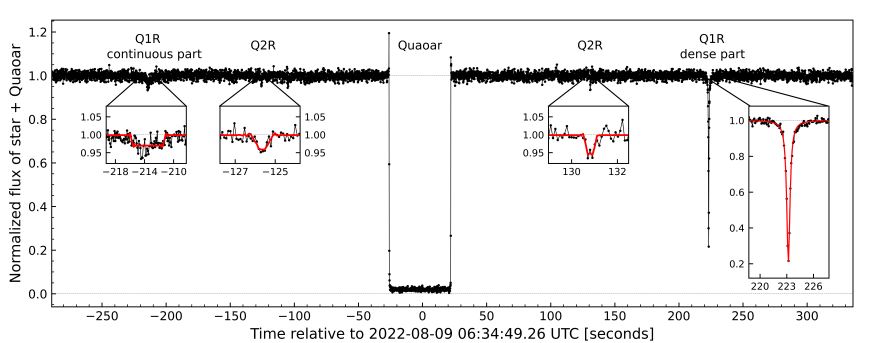
\includegraphics[width=0.95\linewidth]{Tese/pngs/quaoar_test.png}
\caption{Curva de luz da ocultação estelar por Quaoar utilizada no estudo de caso, com o tempo referenciado ao instante 2022-08-09 06:34:49,26 UTC. O \textit{dip} central (anotado como ``Quaoar''), de duração $\approx 48$~s e profundidade $\approx 100\%$, corresponde à ocultação pelo corpo principal. As estruturas secundárias rasas, isoladas nos quatro \textit{insets}, são as assinaturas dos dois anéis denominados Q1R e Q2R em~\citep{Quaoar2023}, sendo Q1R observado em duas porções (parte contínua e parte densa) e Q2R em duas travessias antes e depois do corpo. A linha pontilhada indica o \textit{baseline} ($f_{\mathrm{norm}} = 1$).}
\label{fig:quaoar_curvas}
\end{center}
\end{figure}

\subsection{Aplicação a recortes da curva: sondando os anéis}
\label{sec:quaoar_recortes}

A demonstração mais interessante deste estudo de caso explora justamente a ideia anunciada na Introdução: usar a \textit{pipeline} para \textbf{revisitar uma curva complexa por recortes}, isolando trechos específicos e perguntando ao modelo, janela a janela, se há indício de evento. O dicionário \texttt{CUT\_RANGES} do \textit{script} permite reexecutar a inferência sobre uma janela temporal arbitrária --- a operação é uma única linha (\texttt{cut\_curve(time, flux, t\_ini, t\_fim)}) e pode ser feita interativamente no Debug Console do VS Code, sem retreinar o modelo nem reescrever a \textit{pipeline}.

Tomando a curva Gemini-'Alopeke \textit{Red}-$z$ --- a de maior SNR ---, definiram-se \textbf{seis janelas} que cobrem assinaturas físicas distintas: um trecho de \textit{baseline} sem evento (controle negativo), as duas porções do anel Q1R (contínua e densa), as duas travessias do anel fino Q2R (antes e depois do corpo) e um trecho de ruído visualmente parecido com uma micrococultação, adjacente ao Q2R. A inferência foi aplicada a cada janela com os modelos CatBoost e XGBoost do Experimento~2. A Tabela~\ref{tab:quaoar_recortes} reúne as probabilidades atribuídas.

\begin{table}[htbp]
\centering
\caption{Probabilidade de ocultação $\hat{p}$ atribuída por CatBoost e XGBoost (Exp.~2) a cada recorte da curva Gemini-'Alopeke \textit{Red}-$z$. Janelas em segundos relativos ao instante 2022-08-09 06:34:49,26 UTC.}
\label{tab:quaoar_recortes}
\footnotesize
\begin{tabular}{llcc}
\hline
\textbf{Recorte (janela, s)} & \textbf{Assinatura física} & $\hat{p}$ \textbf{CatBoost} & $\hat{p}$ \textbf{XGBoost} \\
\hline
$-290$ a $-250$ & \textit{baseline} (controle negativo) & 0,029 & 0,0006 \\
$-225$ a $-200$ & Q1R --- parte contínua            & 0,685 & 0,9601 \\
$-129$ a $-114$ & Q2R --- anel fino (real)          & 0,058 & 0,0434 \\
$-109$ a $-099$ & ruído parecido com anel           & 0,005 & 0,0005 \\
$+121$ a $+146$ & Q2R --- anel fino (real)          & 0,456 & 0,0807 \\
$+191$ a $+251$ & Q1R --- parte densa               & 0,987 & 0,9994 \\
\hline
\end{tabular}
\end{table}

A leitura da tabela revela três regimes. \textbf{(i)~Anéis fortes (Q1R):} tanto a parte contínua quanto a densa são detectadas com folga ($\hat{p}=0{,}96$ e $0{,}999$ no XGBoost) --- o sinal é profundo ou longo o bastante para o modelo. \textbf{(ii)~Controle e ruído:} o \textit{baseline} sem evento e o trecho de ruído recebem probabilidades ínfimas ($\hat{p}\approx 6\times10^{-4}$ e $5\times10^{-4}$ no XGBoost), confirmando que o classificador não tem viés pró-positivo. \textbf{(iii)~Anéis finos (Q2R):} aqui está o ponto sutil. Ambos os anéis Q2R recebem veredito \emph{negativo} no limiar padrão $\tau=0{,}5$ ($\hat{p}=0{,}043$ e $0{,}081$ no XGBoost).

À primeira vista, isso pareceria uma falha. Mas o que importa para a revisita de curvas \textbf{não é o valor absoluto da probabilidade, e sim a separação entre eventos e não-eventos}. O anel fino real (Q2R, $\hat{p}=0{,}043$) recebe probabilidade cerca de \textbf{86 vezes maior} do que o trecho de ruído adjacente, de duração comparável ($\hat{p}=0{,}0005$) --- quase duas ordens de grandeza de diferença. Em outras palavras, mesmo ``errando'' a classificação binária, o modelo \emph{ordena corretamente} as janelas: atribui ao anel verdadeiro uma probabilidade pequena em termos absolutos (4--8\%), mas enorme frente à do ruído que mais se parece com uma ocultação (0,05\%). É exatamente esse contraste que um analista revisitando a curva precisa enxergar.

Essa separação é o que torna o \textbf{ajuste de limiar} (Seção~\ref{sec:threshold_tuning}) tão eficaz neste caso. Baixando o limiar para $\tau = 0{,}03$ --- um valor entre as duas escalas de probabilidade ---, os dois anéis Q2R passam a ser corretamente classificados como ocultações, \emph{sem} que o controle ($6\times10^{-4}$) ou o ruído ($5\times10^{-4}$) cruzem o novo limiar. A sensibilidade sobre os quatro eventos físicos da curva (Q1R contínuo, Q1R denso, Q2R$_1$ e Q2R$_2$) sobe de 50\% para 100\%, sem nenhum falso alarme nos dois recortes-controle. Esta é a manifestação prática, em dados reais externos ao treino, do mecanismo de \textit{threshold tuning} apresentado na Seção~\ref{sec:threshold_tuning}. A Figura~\ref{fig:quaoar_recortes} ilustra os seis recortes coloridos sobre a curva, com o veredito em $\tau=0{,}5$ e em $\tau=0{,}03$.

\begin{figure}[htbp]
\begin{center}
	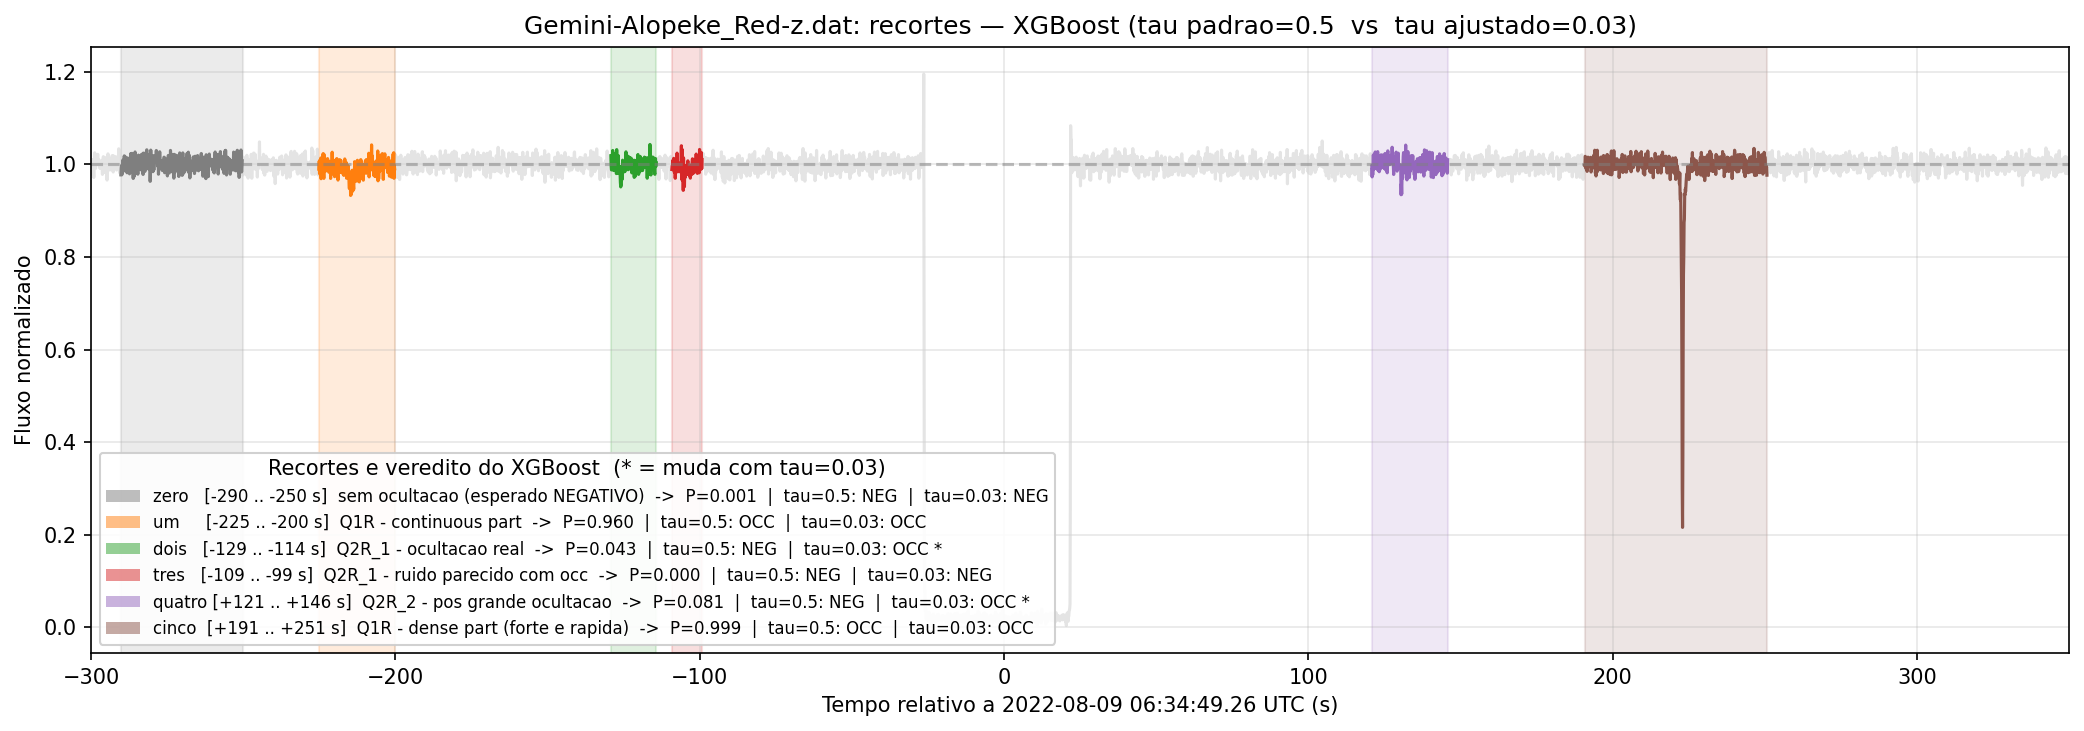
\includegraphics[width=0.95\linewidth]{Tese/pngs/quaoar_recorte_tau_ajustado.png}
\caption{Recortes da curva Gemini-'Alopeke \textit{Red}-$z$ de Quaoar, com o veredito do XGBoost em cada janela colorida. A legenda indica, por recorte, a probabilidade $\hat{p}$ e a classificação no limiar padrão ($\tau=0{,}5$) e no limiar ajustado ($\tau=0{,}03$). Os anéis finos Q2R, negativos em $\tau=0{,}5$, são recuperados em $\tau=0{,}03$, enquanto o controle e o trecho de ruído permanecem corretamente negativos. Tempo relativo a 2022-08-09 06:34:49,26 UTC.}
\label{fig:quaoar_recortes}
\end{center}
\end{figure}

\paragraph{A janela curta não é a causa.} Uma hipótese natural para a baixa probabilidade dos anéis finos seria que as janelas correspondentes (10--25~s) são curtas demais, prejudicando a extração de \textit{features}. Essa hipótese foi testada e \textbf{refutada}: ao ampliar as janelas dos recortes Q2R por um fator $\sim 3$, a probabilidade atribuída pelo XGBoost ao anel real Q2R$_1$ \emph{caiu} de $0{,}043$ para $0{,}035$, e a do Q2R$_2$ caiu de $0{,}081$ para $0{,}029$ --- ou seja, ampliar a janela tornou o veredito negativo ainda mais forte. A explicação é estrutural: o conjunto de \textit{features} é dominado por \textbf{estatísticas globais} da janela (mínimo do Savitzky-Golay, \textit{Max Drawdown}, profundidade, SNR do \textit{dip}). Um \textit{dip} de poucos segundos diluído em dezenas de segundos de \textit{baseline} limpo torna-se um \textit{outlier} estatisticamente desprezível, e o modelo responde com \emph{mais} confiança que se trata de \textit{baseline} puro. A fronteira de detecção é, portanto, regida pela razão entre a duração do \textit{dip} e a duração da janela --- não pelo tamanho absoluto da janela. Esse diagnóstico motiva diretamente as direções de trabalho futuro discutidas no Capítulo~6 (janela deslizante e \textit{features} locais).

\paragraph{Por que XGBoost.} A análise de recortes destaca o XGBoost porque suas probabilidades são mais \textbf{polarizadas}: a razão entre a probabilidade do anel real e a do ruído no Q2R$_1$ é de $\sim 86\times$ no XGBoost, contra $\sim 12\times$ no CatBoost (Tabela~\ref{tab:quaoar_recortes}). Os dois modelos concordam qualitativamente --- ambos detectam o corpo e os anéis fortes e rejeitam controle e ruído ---, mas a maior separação do XGBoost torna o ajuste de limiar mais robusto. Isso é coerente com a leve vantagem do XGBoost no teste em curvas exclusivamente reais (Experimento~3). A subseção anterior, sobre a curva completa, usou o CatBoost-Exp.~2; aqui, ambos classificam o corpo principal com $\hat{p}>0{,}99$, e o XGBoost é preferido apenas para a discussão dos eventos sutis.

\subsection{Interpretação}

O estudo de caso reforça, na prática, quatro conclusões dos experimentos formais:

\begin{enumerate}
	\item \textbf{Generalização para dados externos:} mesmo treinado em curvas predominantemente sintéticas e oriundas dos catálogos VizieR/Grupo do Rio, o modelo do Experimento~2 classifica corretamente registros de uma campanha observacional distinta, em três bandas espectrais e dois telescópios diferentes.
	\item \textbf{Robustez a complexidade morfológica:} a presença de estruturas secundárias na curva (anéis) não confunde o classificador, que mantém probabilidades $> 0{,}99$ para o evento principal.
	\item \textbf{Capacidade de triagem de eventos sutis por recorte:} ainda que os anéis finos Q2R fiquem abaixo do limiar padrão, o modelo lhes atribui probabilidade até $\sim 86\times$ maior do que a um trecho de ruído semelhante. Essa separação --- e não o valor absoluto --- é o que permite recuperá-los com um simples ajuste de limiar, validando a \textit{pipeline} como ferramenta para revisitar curvas em busca de descobertas.
	\item \textbf{Utilidade operacional:} o procedimento --- leitura do \texttt{.dat}, limpeza, recorte opcional e inferência --- é executado em segundos e pode ser incorporado a campanhas reais com modificação mínima.
\end{enumerate}

Como limitação, vale registrar que se trata de um \textit{n} pequeno (três curvas, todas do mesmo evento) e que os modelos atuais não estão otimizados para detectar separadamente os eventos de anel: o ajuste de limiar resolve o caso prático, mas não substitui melhorias estruturais como janela deslizante, \textit{features} locais ou classificação multi-classe. Uma avaliação sistemática nesse regime --- inclusive incorporando dados de campanhas similares no banco de treino --- é uma das direções recomendadas no Capítulo~6.

% -----------------------------------------------------------------------------
\section{Comparação entre os experimentos}
\label{sec:comparacao}

A Tabela~\ref{tab:comparacao_f1} permite uma visão comparativa do F1-score por modelo nos seis experimentos realizados.

\begin{table}[htbp]
\centering
\caption{Comparação do F1-score entre os seis experimentos, por modelo. Exp.~1: 28 \textit{features}; Exp.~2: 11 \textit{features} (ablação combinada); Exp.~3: teste somente em curvas reais; Exp.~4: 14 \textit{features}; Exp.~5: 13 \textit{features}; Exp.~6: 12 \textit{features} (sem \texttt{kmeans}). Todos com divisão 80/20, exceto o Exp.~3 (treino 65/35, teste real).}
\label{tab:comparacao_f1}
\footnotesize
\begin{tabular}{lcccccc}
\hline
\textbf{Modelo} & \textbf{Exp. 1} & \textbf{Exp. 2} & \textbf{Exp. 3} & \textbf{Exp. 4} & \textbf{Exp. 5} & \textbf{Exp. 6} \\
 & \scriptsize{28 f.} & \scriptsize{11 f.} & \scriptsize{teste real} & \scriptsize{14 f.} & \scriptsize{13 f.} & \scriptsize{12 f.} \\
 & \scriptsize{80/20} & \scriptsize{80/20} & \scriptsize{65/35} & \scriptsize{80/20} & \scriptsize{80/20} & \scriptsize{80/20} \\
\hline
Random Forest   & \textbf{0,9937} & 0,9874 & 0,9803 & 0,9874 & \textbf{0,9905} & \textbf{0,9906} \\
XGBoost         & 0,9844 & \textbf{0,9906} & \textbf{0,9821} & 0,9875 & 0,9843 & \textbf{0,9906} \\
CatBoost        & 0,9906 & 0,9905 & 0,9784 & \textbf{0,9906} & 0,9873 & 0,9874 \\
Regressão Log.  & 0,9873 & 0,9841 & 0,9746 & 0,9873 & 0,9873 & 0,9873 \\
\hline
\end{tabular}
\end{table}

Cinco observações principais emergem da análise conjunta:

\begin{enumerate}
	\item \textbf{Estabilidade entre conjuntos de \textit{features}.} A redução de 28 (Experimento 1) para 14 \textit{features} (Experimento 4) preserva o desempenho, com F1 entre 0,98 e 0,99.

	\item \textbf{Impacto da remoção de \texttt{Feature\_Savgol\_Min}.} No Experimento 5 (13 \textit{features}), o Random Forest lidera com F1 = 0,9905; a remoção dessa \textit{feature} não causa degradação acentuada.

	\item \textbf{Dispensabilidade do K-Means.} Nos Experimentos 6 e 2, a remoção de \texttt{kmeans\_centroid\_dist} (e, no Exp.~2, também de \texttt{Feature\_Savgol\_Min}) não degrada o desempenho: XGBoost e CatBoost mantêm F1 $\geq 0{,}990$. A colinearidade funcional com \texttt{Feature\_Savgol\_std} explica essa redundância.

	\item \textbf{Generalização em curvas reais.} O Experimento 3 (teste somente em curvas reais) mostra queda de $\approx$2~pp em F1, com AUC-ROC ainda acima de 0,995, indicando que as \textit{features} capturam sinal real e não apenas artefatos da distribuição sintética.

	\item \textbf{AUC-ROC.} Em todos os experimentos com teste misto (todos exceto o Experimento 3), a AUC-ROC permanece $\geq 0{,}9995$; no Experimento 3, $\geq 0{,}9959$.
\end{enumerate}

As Figuras~\ref{fig:ROC1} e~\ref{fig:ROC7} apresentam as curvas ROC dos dois cenários mais informativos --- a linha de base em dados mistos (Experimento~1) e o teste exclusivamente em curvas reais (Experimento~3) ---, ilustrando o contraste entre a separação quase perfeita no primeiro e a degradação leve, porém ainda excelente, no segundo. As curvas ROC dos demais experimentos estão reunidas no Apêndice~\ref{ap:experimentos}.

\begin{figure}[htbp]
\begin{center}
	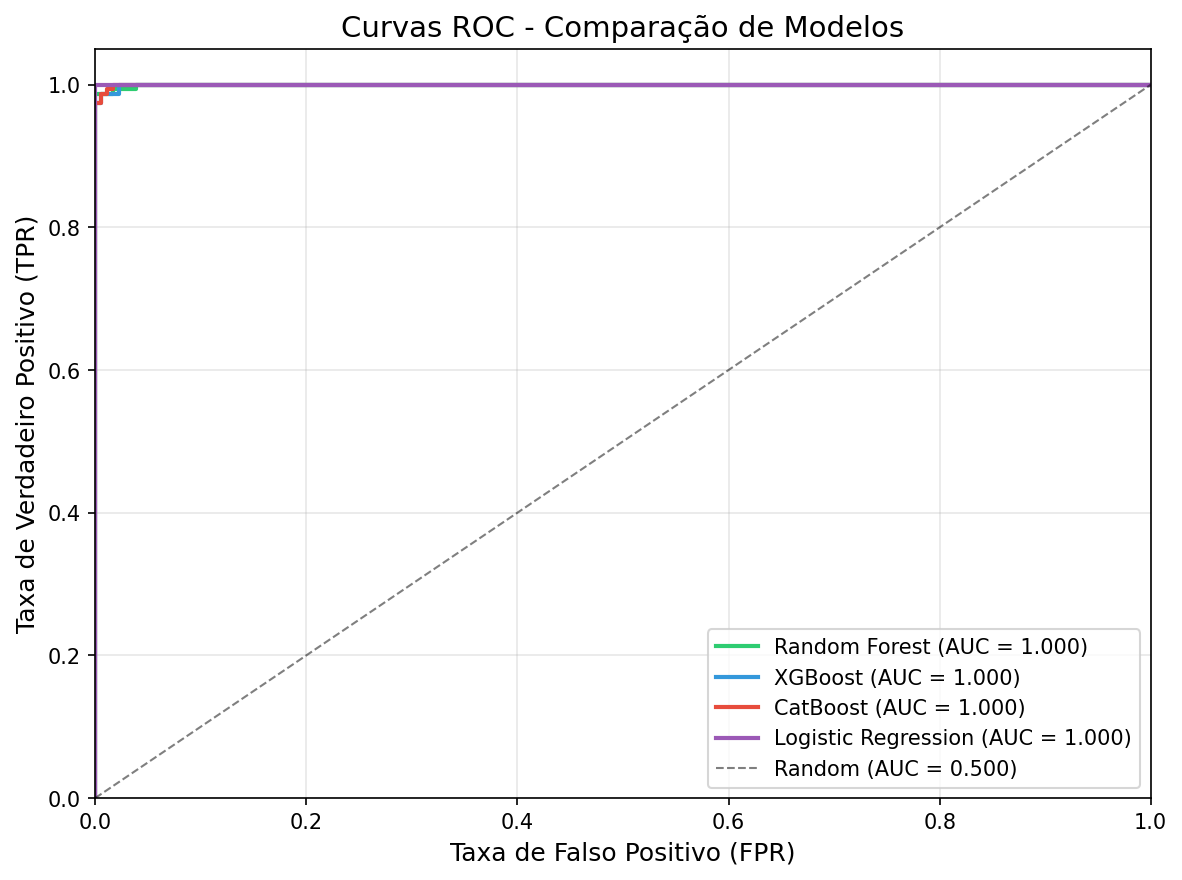
\includegraphics[width=0.7\textwidth]{Tese/pngs/exp1/roc_curves.png}
\caption{Curvas ROC --- Experimento 1 (28 \textit{features}).}
\label{fig:ROC1}
\end{center}
\end{figure}

\begin{figure}[htbp]
\begin{center}
	
\includegraphics[width=0.7\textwidth]{Tese/pngs/exp7/roc_curves.png}
\caption{Curvas ROC --- Experimento 3 (teste somente em curvas reais).}
\label{fig:ROC7}
\end{center}
\end{figure}

\subsection{Análise de importância das \textit{features}}

A Figura~\ref{fig:feature_importance_1} apresenta os gráficos de importância de variáveis para os quatro modelos no Experimento~1 (conjunto completo de 28 \textit{features}); as figuras análogas dos demais experimentos estão no Apêndice~\ref{ap:experimentos}. A interpretação dos valores deve considerar as diferenças metodológicas discutidas na Seção~\ref{sec:feature_importance_metodologia}: o eixo horizontal varia de 0 a $\approx$0,25 no Random Forest (MDI normalizado para soma~1), de 0 a $\approx$0,15 no XGBoost (\textit{weight} normalizado), de 0 a $\approx$30 no CatBoost (\textit{PredictionValuesChange} normalizado para soma~100), e de 0 a $\approx$4 na Regressão Logística ($|\beta_j|$ sem normalização).

Em todos os experimentos e modelos, as variáveis mais relevantes consistentemente incluem:

\begin{itemize}
	\item \texttt{Feature\_Savgol\_Min} e \texttt{Max\_Drawdown}: capturam diretamente a magnitude da queda de fluxo, que é a assinatura primária de uma ocultação.
	\item \texttt{kmeans\_centroid\_dist}: a distância entre os centróides do K-Means identifica a presença de dois regimes no fluxo (dentro e fora do dip), sendo altamente discriminativa.
	\item \texttt{Occ\_depth} e \texttt{Occ\_SNR\_dip}: quantificam a profundidade e a razão sinal-ruído do evento segundo critérios observacionais.
	\item \texttt{MinLogP\_Ttest} e \texttt{MinLogP\_KS}: os testes estatísticos entre quartis detectam heterogeneidade no fluxo, que é esperada em curvas com ocultação.
\end{itemize}

\begin{figure}[p]
\centering
\noindent\textbf{Experimento 1 (28 \textit{features}).}\\[0.5em]
\begin{minipage}[t]{0.48\textwidth}
	\centering
	
\includegraphics[width=\linewidth]{Tese/pngs/exp1/feature_importance_logistic_regression.png}
	\vspace{0.3em}
	\small (a) Regressão Log.
\end{minipage}\hfill
\begin{minipage}[t]{0.48\textwidth}
	\centering
	
\includegraphics[width=\linewidth]{Tese/pngs/exp1/feature_importance_random_forest.png}
	\vspace{0.3em}
	\small (b) Random Forest
\end{minipage}\\[1em]
\begin{minipage}[t]{0.48\textwidth}
	\centering
	
\includegraphics[width=\linewidth]{Tese/pngs/exp1/feature_importance_xgboost.png}
	\vspace{0.3em}
	\small (c) XGBoost
\end{minipage}\hfill
\begin{minipage}[t]{0.48\textwidth}
	\centering
	
\includegraphics[width=\linewidth]{Tese/pngs/exp1/feature_importance_catboost.png}
	\vspace{0.3em}
	\small (d) CatBoost
\end{minipage}\\[0.5em]
\caption{Importância de variáveis por modelo --- Experimento 1 (28 \textit{features}). (a) Regressão Logística, (b) Random Forest, (c) XGBoost, (d) CatBoost.}
\label{fig:feature_importance_1}
\end{figure}

As figuras análogas para os Experimentos 4 e 5, que permitem acompanhar como a importância relativa das variáveis se redistribui à medida que o conjunto é reduzido, estão reunidas no Apêndice~\ref{ap:experimentos}.

A viabilidade da \textit{feature} \texttt{kmeans\_centroid\_dist} como variável discriminativa é corroborada pela análise exploratória dos dados: curvas positivas (com ocultação) concentram-se em valores mais altos de distância entre centróides, enquanto curvas negativas concentram-se em valores menores. A separação entre as duas distribuições confirma que a distância entre centróides captura eficazmente a presença de dois regimes na série temporal.
% Se disponível nos outputs do pipeline, descomentar a figura abaixo:
%\begin{figure}[htbp]
%\begin{center}
%	
\includegraphics[width=0.85\linewidth]{Tese/pngs/exp1/histograma_kmeans_por_classe.png}
%\caption{Histograma da \textit{feature} \texttt{kmeans\_centroid\_dist} por classe.}
%\label{fig:histograma_kmeans}
%\end{center}
%\end{figure}

% -----------------------------------------------------------------------------
\section{Validação cruzada estratificada}
\label{sec:cross_validation}

Os resultados das seções anteriores baseiam-se em uma única divisão treino/teste por experimento. Isso é útil para comparar modelos sob as mesmas condições, mas não diz o quanto o desempenho \emph{varia} se mudarmos a divisão dos dados. Para medir essa variabilidade, repetimos a avaliação cinco vezes, com partições diferentes --- procedimento conhecido como \textbf{validação cruzada com $k=5$ dobras}.

O procedimento é simples. Primeiro, embaralha-se o conjunto e divide-se em 5 partes (as ``dobras'') de tamanho parecido. Em seguida, faz-se cinco rodadas: em cada uma, quatro dobras servem de treino e a quinta de teste, alternando qual dobra é a de teste, de modo que toda curva é avaliada exatamente uma vez. As partições são \textbf{estratificadas} (cada dobra mantém a mesma proporção entre as duas classes, positiva e negativa --- continua sendo um problema binário) e respeitam o \textbf{agrupamento por curva} (todos os segmentos recortados de uma mesma curva ficam na mesma dobra, para que o modelo nunca seja testado em um pedaço de uma curva que viu no treino, o que inflaria artificialmente o desempenho). Em cada rodada, os quatro modelos são treinados e avaliados de forma independente, registrando-se F1-score, precisão, sensibilidade e AUC-ROC. O resultado final é a \textbf{média $\pm$ desvio padrão} dessas métricas sobre as cinco dobras: a média estima o desempenho típico e o desvio padrão, a sua variabilidade.

A Tabela~\ref{tab:cross_validation} apresenta a média e o desvio padrão das métricas na validação cruzada estratificada 5-fold (Experimento~5, 13 \textit{features}).

\begin{table}[htbp]
\centering
\small
\caption{Validação cruzada estratificada ($k=5$): média $\pm$ desvio padrão das métricas por modelo (Experimento~5).}
\label{tab:cross_validation}
\begin{tabular}{@{}lccccc@{}}
\hline
\textbf{Modelo} & \textbf{Acurácia} & \textbf{Precisão} & \textbf{Sensibilidade} & \textbf{F1} & \textbf{AUC-ROC} \\
\hline
CatBoost          & $0{,}9876 \pm 0{,}0067$ & $0{,}9912 \pm 0{,}0034$ & $0{,}9825 \pm 0{,}0148$ & $0{,}9868 \pm 0{,}0072$ & $0{,}9993 \pm 0{,}0005$ \\
XGBoost           & $0{,}9864 \pm 0{,}0058$ & $0{,}9888 \pm 0{,}0090$ & $0{,}9825 \pm 0{,}0167$ & $0{,}9856 \pm 0{,}0062$ & $0{,}9992 \pm 0{,}0008$ \\
Regressão Log.    & $0{,}9846 \pm 0{,}0097$ & $0{,}9911 \pm 0{,}0057$ & $0{,}9763 \pm 0{,}0172$ & $0{,}9836 \pm 0{,}0104$ & $0{,}9986 \pm 0{,}0016$ \\
Random Forest     & $0{,}9840 \pm 0{,}0068$ & $0{,}9826 \pm 0{,}0051$ & $0{,}9838 \pm 0{,}0129$ & $0{,}9831 \pm 0{,}0072$ & $0{,}9992 \pm 0{,}0007$ \\
\hline
\end{tabular}
\end{table}

A validação cruzada cumpre dois objetivos: (1)~confirmar que o desempenho elevado observado nos experimentos anteriores não é artefato de uma partição favorável dos dados; e (2)~fornecer desvios padrão que permitam avaliar se as diferenças entre modelos são significativas ou estão dentro da flutuação estatística. Se o desvio padrão do F1 for pequeno (e.g., $< 0{,}01$), isso reforça a conclusão de que o desempenho é robusto; se for grande, pode indicar sensibilidade à composição do conjunto de teste.

\subsection{Teste de McNemar entre modelos}
\label{sec:mcnemar}

Para determinar se as diferenças de desempenho entre pares de modelos são \textbf{estatisticamente significativas} --- e não meras flutuações amostrais --- aplicou-se o \textbf{teste de McNemar} \citep{McNemarOrig1947}, cujo uso adequado em comparação de classificadores é discutido por \citet{McNemar1947}. Esse teste é apropriado para comparar dois classificadores avaliados no mesmo conjunto de teste: constrói-se uma tabela $2 \times 2$ de concordância/discordância entre as predições dos dois modelos, e testa-se se os padrões de discordância são simétricos.

Sejam $b$ o número de exemplos que o modelo~A erra e o modelo~B acerta, e $c$ o número de exemplos que o modelo~A acerta e o modelo~B erra. A estatística de McNemar (com correção de continuidade) é:
\begin{equation}
\chi^2 = \frac{(|b - c| - 1)^2}{b + c},
\end{equation}
que segue uma distribuição $\chi^2$ com 1 grau de liberdade sob a hipótese nula $H_0: b = c$ (os modelos têm a mesma taxa de erro). Se $p < 0{,}05$, rejeita-se $H_0$ e conclui-se que a diferença é significativa.

A Tabela~\ref{tab:mcnemar} apresenta os resultados do teste de McNemar entre pares de modelos (Experimento~4, 14 \textit{features}).

\begin{table}[htbp]
\centering
\small
\caption{Teste de McNemar entre pares de modelos (Experimento~4). $b$: apenas A acerta; $c$: apenas B acerta. $p < 0{,}05$ indicaria diferença significativa; nenhum par é significativo ($\alpha = 0{,}05$).}
\label{tab:mcnemar}
\begin{tabular}{@{}llcccl@{}}
\hline
\textbf{Modelo A} & \textbf{Modelo B} & $b$ & $c$ & $\chi^2$ & $p$ \\
\hline
RF & XGBoost       & 1 & 1 & 0,50 & 0,4795 \\
RF & CatBoost      & 1 & 2 & 0,00 & 1,0000 \\
RF & Reg. Log.     & 2 & 2 & 0,25 & 0,6171 \\
XGBoost & CatBoost  & 0 & 1 & 0,00 & 1,0000 \\
XGBoost & Reg. Log. & 3 & 3 & 0,17 & 0,6831 \\
CatBoost & Reg. Log.& 3 & 2 & 0,00 & 1,0000 \\
\hline
\end{tabular}
\end{table}

\textbf{Conclusão:} Nenhum par de modelos apresenta diferença estatisticamente significativa; os quatro classificadores podem ser considerados equivalentes no conjunto de teste deste experimento.

Em cenários de alto desempenho (F1 $> 0{,}97$), é comum que os valores de $b$ e $c$ sejam pequenos, o que pode tornar o teste pouco potente. Se o McNemar indicar que as diferenças \textbf{não} são significativas para a maioria dos pares, isso sugere que os modelos são equivalentes no contexto deste \textit{dataset} e que a escolha entre eles pode ser guiada por critérios secundários (interpretabilidade, velocidade de inferência, facilidade de implantação).

% -----------------------------------------------------------------------------
\section{Discussão dos resultados}
\label{sec:discussao}

\subsection{Desempenho e generalização}

Os resultados dos seis experimentos indicam que a \textit{pipeline} de detecção automatizada atinge \textbf{desempenho elevado e estável} na classificação binária de curvas de luz: F1-score entre 0,974 e 0,994 no teste misto (todos os experimentos, exceto o Experimento~3) e entre 0,975 e 0,982 no teste exclusivamente em curvas reais (Experimento~3); AUC-ROC superior a 0,995 em todos os cenários. Esse patamar é compatível com o objetivo de desenvolver uma ferramenta de triagem que permita priorizar curvas candidatas a análise detalhada.

\textbf{Sobre a possibilidade de \textit{overfitting}.} Todas as métricas referem-se ao \textbf{conjunto de teste}; portanto, o desempenho descrito é uma estimativa da capacidade de generalização. Vários indícios sugerem que o \textit{overfitting} não domina os resultados: (i)~as métricas são estáveis entre os seis experimentos e quatro modelos; (ii)~a redução de 28 para 14 ou 11 \textit{features} preserva ou melhora ligeiramente o F1; (iii)~foram empregados mecanismos de regularização (Ridge na Regressão Logística, \texttt{class\_weight='balanced'}, limites de profundidade nos \textit{ensembles}); (iv)~a validação cruzada 5-fold (Seção~\ref{sec:cross_validation}) apresenta desvios padrão pequenos ($\approx$0,006--0,010 em F1). A confirmação definitiva de boa generalização exigiria validação em dados independentes de outros catálogos.

\subsection{Análise de redundância}

A análise de redundância (Seção~\ref{sec:features_redundancia}) identificou 15 variáveis redundantes ou com baixo poder discriminativo. A comparação entre os Experimentos 1 (28 \textit{features}) e 4 (14 \textit{features}) demonstra empiricamente que a remoção dessas variáveis não prejudica --- e pode até melhorar --- o desempenho dos classificadores. Isso é consistente com a teoria de \textit{machine learning}: variáveis redundantes aumentam a dimensionalidade do espaço de entrada sem acrescentar informação, podendo elevar a variância dos modelos.

A importância da \textit{feature} \texttt{Feature\_Savgol\_Min} é coerente com a física do problema: em uma ocultação, o fluxo normalizado cai durante o intervalo em que a estrela está atrás do corpo; o mínimo da série suavizada localiza esse patamar e tende a ser mais baixo em curvas com evento do que em curvas ruidosas sem ocultação. A queda de desempenho ao remover essa variável (Experimento 5) reforça seu papel discriminativo.

\subsection{Interpretação da importância das \textit{features}}

A concordância entre os quatro modelos quanto às \textit{features} mais importantes --- \texttt{Feature\_Savgol\_Min}, \texttt{Max\_Drawdown}, \texttt{kmeans\_centroid\_dist} e as métricas observacionais de profundidade e SNR --- oferece confiança de que essas variáveis capturam as assinaturas físicas relevantes de uma ocultação: queda de fluxo (profundidade), localização temporal da queda (duração), e separação entre os níveis de fluxo dentro e fora do evento (bimodalidade via K-Means). A coerência entre modelos de naturezas distintas (linear vs.\ árvores, \textit{bagging} vs.\ \textit{boosting}) reforça a robustez dessa interpretação.

O estudo de ablação (Seção~\ref{sec:ablation_kmeans}) acrescenta uma nuance importante: embora \texttt{kmeans\_centroid\_dist} seja consistentemente apontada como a \textit{feature} mais importante pelos modelos de árvore --- chegando a 63\% de importância no XGBoost ---, sua remoção não degrada o desempenho. Isso demonstra que a \textbf{importância atribuída por algoritmos baseados em árvore não é sinônimo de insubstituibilidade}: uma \textit{feature} pode concentrar alta importância simplesmente por oferecer um ponto de corte mais eficiente, enquanto outras variáveis colineares podem compensar sua ausência redistribuindo a capacidade preditiva. Esse resultado tem implicação prática direta: o \textit{pipeline} pode ser simplificado pela remoção do passo de K-Means sem perda de qualidade.

\subsection{Custo assimétrico e ajuste de limiar}

Em um cenário real de triagem, o custo de perder uma ocultação genuína (falso negativo) supera amplamente o custo de revisar uma curva sem evento (falso positivo). A Seção~\ref{sec:threshold_tuning} demonstra que essa assimetria pode ser incorporada à \textit{pipeline} sem retreinamento, simplesmente reduzindo o limiar de decisão $\tau$. Essa abordagem explora o fato de que os modelos produzem probabilidades, não apenas rótulos binários, e que a separabilidade elevada entre as classes (AUC-ROC $\geq 0{,}998$) garante que a precisão se mantenha aceitável mesmo em patamares de sensibilidade próximos de 100\%. A possibilidade de ajuste de limiar em pós-processamento é uma vantagem direta da formulação probabilística adotada, e confere à \textit{pipeline} flexibilidade para operar em diferentes cenários de custo sem modificação dos modelos.

\subsection{Limitações}

\begin{enumerate}
	\item O \textit{ground truth} (rótulos positivo/negativo) provém dos catálogos VizieR e Grupo do Rio; erros ou inconsistências de rotulagem podem afetar treinamento e avaliação.
	\item Os experimentos individuais utilizam uma única divisão treino/teste fixa por configuração. A validação cruzada estratificada (Seção~\ref{sec:cross_validation}) e o teste de McNemar (Seção~\ref{sec:mcnemar}) fornecem estimativas de variabilidade e testes de significância; uma validação cruzada repetida com múltiplas sementes fortaleceria as conclusões.
	\item A generalização para outros catálogos, condições de observação ou objetos ocultantes diferentes dos presentes no banco de dados não foi avaliada sistematicamente neste trabalho.
	\item O \textit{dataset} é parcialmente sintético (cerca de 78\% dos negativos); o Experimento~3 mostra que o desempenho em curvas exclusivamente reais é ligeiramente menor, embora ainda elevado (AUC $> 0{,}995$).
\end{enumerate}

\subsection{Recomendações para trabalhos futuros}

\begin{itemize}
	\item Validação em conjuntos de dados independentes (outros catálogos ou campanhas observacionais).
	\item Análise de significância via validação cruzada repetida, com reporte de média e desvio padrão do F1-score.
	\item Estudo de \textit{features} baseadas em modelos físicos mais sofisticados (difração de Fresnel, opacidade parcial), que poderiam melhorar a discriminação em eventos de baixo SNR.
	\item Aplicação da \textit{pipeline} a dados de campanhas observacionais específicas, como as curvas de luz do objeto transnetuniano Quaoar, para validação em cenário real de uso.
\end{itemize}

A hipótese de pesquisa formulada na Introdução --- de que é possível obter desempenho comparável a abordagens manuais ou baseadas em redes convolucionais usando \textit{features} clássicas e \textit{ensembles} de árvores, com vantagem de interpretabilidade --- é corroborada pelos resultados obtidos nos seis experimentos. As análises de ablação da \textit{feature} K-Means (Seção~\ref{sec:ablation_kmeans}) e de generalização em curvas reais (Seção~\ref{sec:generalizacao_real}) reforçam essa conclusão ao demonstrar que o desempenho elevado é robusto à simplificação do conjunto de variáveis (28 $\to$ 11 \textit{features}) e ao teste exclusivo em dados reais, evidenciando que o \textit{feature engineering} baseado em domínio é o fator determinante da qualidade da classificação.
